%%
%% This is file `sample-manuscript.tex',
%% generated with the docstrip utility.
%%
%% The original source files were:
%%
%% samples.dtx  (with options: `manuscript')
%% 
%% IMPORTANT NOTICE:
%% 
%% For the copyright see the source file.
%% 
%% Any modified versions of this file must be renamed
%% with new filenames distinct from sample-manuscript.tex.
%% 
%% For distribution of the original source see the terms
%% for copying and modification in the file samples.dtx.
%% 
%% This generated file may be distributed as long as the
%% original source files, as listed above, are part of the
%% same distribution. (The sources need not necessarily be
%% in the same archive or directory.)
%%
%% The first command in your LaTeX source must be the \documentclass command.
%%%% Small single column format, used for CIE, CSUR, DTRAP, JACM, JDIQ, JEA, JERIC, JETC, PACMCGIT, TAAS, TACCESS, TACO, TALG, TALLIP (formerly TALIP), TCPS, TDSCI, TEAC, TECS, TELO, THRI, TIIS, TIOT, TISSEC, TIST, TKDD, TMIS, TOCE, TOCHI, TOCL, TOCS, TOCT, TODAES, TODS, TOIS, TOIT, TOMACS, TOMM (formerly TOMCCAP), TOMPECS, TOMS, TOPC, TOPLAS, TOPS, TOS, TOSEM, TOSN, TQC, TRETS, TSAS, TSC, TSLP, TWEB.
% \documentclass[acmsmall]{acmart}

%%%% Large single column format, used for IMWUT, JOCCH, PACMPL, POMACS, TAP, PACMHCI
% \documentclass[acmlarge,screen]{acmart}

%%%% Large double column format, used for TOG
% \documentclass[acmtog, authorversion]{acmart}

%%%% Generic manuscript mode, required for submission
%%%% and peer review
\documentclass[manuscript,screen]{acmart}

%%
%% \BibTeX command to typeset BibTeX logo in the docs
\AtBeginDocument{%
  \providecommand\BibTeX{{%
    \normalfont B\kern-0.5em{\scshape i\kern-0.25em b}\kern-0.8em\TeX}}}

%% Rights management information.  This information is sent to you
%% when you complete the rights form.  These commands have SAMPLE
%% values in them; it is your responsibility as an author to replace
%% the commands and values with those provided to you when you
%% complete the rights form.
%\setcopyright{acmcopyright}
\copyrightyear{2020}
%\acmYear{2020}
%\acmDOI{10.1145/1122445.1122456}

%% These commands are for a PROCEEDINGS abstract or paper.
%\acmConference[Woodstock '18]{Woodstock '18: ACM Symposium on Neural
 % Gaze Detection}{June 03--05, 2018}{Woodstock, NY}
%\acmBooktitle{Woodstock '18: ACM Symposium on Neural Gaze Detection,
 % June 03--05, 2018, Woodstock, NY}
%\acmPrice{15.00}
%\acmISBN{978-1-4503-XXXX-X/18/06}
\usepackage{booktabs}
\usepackage{bbding}
\usepackage{pifont}
\usepackage{wasysym}
\usepackage{amssymb}
%%
%% end of the preamble, start of the body of the document source.
\begin{document}

%%
%% The "title" command has an optional parameter,
%% allowing the author to define a "short title" to be used in page headers.
\title{A Survey of AR Piano Prototypes}

%%
%% The "author" command and its associated commands are used to define
%% the authors and their affiliations.
%% Of note is the shared affiliation of the first two authors, and the
%% "authornote" and "authornotemark" commands
%% used to denote shared contribution to the research.
\author{Jordan Aiko Deja}
%\authornote{Both authors contributed equally to this research.}
\email{jordan.deja@famnit.upr.si}
\orcid{1234-5678-9012}
\affiliation{%
  \institution{University of Primorska}
  \city{Koper}
  \country{Slovenia}
  \postcode{6000}
}

%\author{Matjaž Kljun and Klen Čopič Pucihar}
%\affiliation{%
%  \institution{Advisors}
%  \city{Koper}
 % \postcode{6000}}
%\email{\{matjaz.kljun, klen.copic\}@famnit.upr.si}

%\author{Klen Čopič Pucihar}
%\affiliation{%
%  \institution{University of Primorska}
 % \city{Koper}
  %\country{Slovenia}
  %\postcode{6000}}
%\email{klen.copic@famnit.upr.si}

%%
%% By default, the full list of authors will be used in the page
%% headers. Often, this list is too long, and will overlap
%% other information printed in the page headers. This command allows
%% the author to define a more concise list
%% of authors' names for this purpose.
\renewcommand{\shortauthors}{Deja, et al.}
%%
%% The abstract is a short summary of the work to be presented in the
%% article.
\begin{abstract}
\textbf{Abstract:} Humans have been using and learning the piano for over 3 centuries. In the last 15 years, several Augmented Reality (AR) piano prototypes that support learning have been introduced. Why are we still building these prototypes? What do these systems lack? In this paper, we present a systematic review of AR piano prototypes developed within the recent years. We review the different innovations they present and organise them into contribution categories. We will then discuss the impact of these contributions and recommend directions for future work towards designing better AR piano prototypes and conducting user studies.
\end{abstract}
%%
%% The code below is generated by the tool at http://dl.acm.org/ccs.cfm.
%% Please copy and paste the code instead of the example below.
%%
\begin{CCSXML}
<ccs2012>
   <concept>
       <concept_id>10003120.10003138.10011767</concept_id>
       <concept_desc>Human-centered computing~Empirical studies in ubiquitous and mobile computing</concept_desc>
       <concept_significance>500</concept_significance>
       </concept>
 </ccs2012>
\end{CCSXML}
\ccsdesc[500]{Human-centered computing~Empirical studies in ubiquitous and mobile computing}
%%
%% Keywords. The author(s) should pick words that accurately describe
%% the work being presented. Separate the keywords with commas.
\keywords{augmented reality, piano, meta-analysis, prototypes}
%%
%% This command processes the author and affiliation and title
%% information and builds the first part of the formatted document.
\maketitle

\section{Introduction}
In around the year 1700, the piano, an elegant yet complex to use musical instrument was invented. Since then, humans have been designing innovations improving the experiences of learning and playing the piano. Several technology interventions have been introduced to assist in these scenarios. As these contributions are presented, changes in the way humans use the piano and technology also take place. This is because of the affordances affecting users that go with these technologies. One of these innovations is through Augmented Reality (AR). The earliest known prototype designed with AR came in the late 90s in the form of a musical keyboard display with keyboard input method \cite{breitweiser1996musical}. This along with other AR prototypes rode the waves of the Information era, with the boom of the World Wide Web, the emergence of the millennium bug, higher resolution graphics, stronger processors and better tracking algorithms among many others. Since then, as several AR piano prototypes have been developed, key innovations have shifted focus as well jumping from one technology to other (e.g. overlaying graphics to optimization to teaching modes). As these innovations shift focus from one to the other, human experiences are also reshaped by these changes. 

\citet{dede1996evolution} contends that technological media (such as computers) provide affordances that play an important role in the use and teaching with technology. Therefore, it is important to study how learning a music instrument augmented with digital technology and how such innovations can be maximized to improve and sustain piano learning experiences. A study by \citet{tamim2011forty} shows us that the use of technology can help learners improve their over-all performance. We believe that the same approach can be made applicable in piano learning as well. This is why we think that several prototypes and technologies have been developed for the piano. 


\subsection{Objectives}

Several technologies have enabled the creation of prototypes, learning modes and interactive spaces. Over the last 20 years, we have observed progress in hardware computing power, tracking of elements in real-time (such has hand, object tracking) and in authoring AR tools, plug-ins and applications. These technologies are already seen and applied in several settings such as in tourism \cite{kounavis2012enhancing}, learning \cite{santos2013augmented}, manufacturing \cite{thomas1992augmented}, pilot training \cite{macchiarella2004augmented} and many others. As a first goal, this paper aims to review the different trends and categories that have improved AR experiences with special emphasis to the piano. Even though there have been several AR piano prototypes in current literature, we believe that only a few are developed with focus on improving how piano novices learn (and towards having sustainable, meaningful learning experiences). The different novel contributions in piano AR have been measured to be effective based on several metrics such as registration speed, quality of graphics, and observed learner performance. These studies have been written with a distinct context in mind. As such, replicating these studies will depend on various factors such as: accessibility of required hardware, difficulty of recreating assets, available open-source libraries and willing participants for user studies. As a second goal, we intend to guide researchers on possible directions towards introducing novel contributions in AR piano prototypes. We shall do this by summarizing the state-of-the-art implementation and evaluation of included literature. Then, we enumerate recommendations for learning piano with AR and discuss relevant innovations and models that can support these recommendations. 

\subsection{Organization}
The paper is organized as follows: Section 2 discusses our definition of Augmented Reality (AR) piano prototypes and a background on the piano learning process. Section 3 describes our methods for qualitative analysis. Section 4 discusses the results of our analysis of the trends in AR piano prototypes designed throughout the years. Section 5 discusses the results of our qualitative analysis of AR piano prototypes covering state-of-the-art contributions (in the design, engineering and content). We organise these strategies into categories such as hand tracking, visualisations, agents and tutors, and learning modes in Section 5. We also look at the evaluation aspect of these studies and the analyses that go with them as covered in Section 6. Lastly, Section 7 concludes this paper with our recommendation for future AR piano prototypes. 


\section{Background}
%\subsection{Piano Learning}
How do people learn the piano? what are the different stages of learning the piano? what stages in piano learning have been augmented by technology? what are the existing gaps in this process? How much virtuality (in miligram's continuum) has been included in piano? 

%\subsection{Augmented Reality Piano Prototypes}
Augmented Reality
Augmented reality piano teaching systems
Design Factors affecting augmented reality piano teaching systems (hardware, software, content)

\section{Method}

We did a literature review following the \textit{Preferred Reporting Items for Systematic Reviews and Meta-Analyses} technique, also known as \textbf{PRISMA} \cite{moher2009preferred}. The work of \citet{santos2013augmented} which has reviewed AR learning environments has applied PRISMA techniques as well. This guided us further on how to analyse and review AR prototypes for this specific context. The approach included a  qualitative-analysis phase that aims to review these innovations in a specific context. The methodology for this systematic review is as follows: 

\subsection{Search for Prototypes}
\label{subsec: search}
We did a literature search between March to August 2020 in several digital libraries such as Google Scholar, ACM Digital Library and IEEE Xplore Digital Library. The search strings used where:
\begin{enumerate}
    \item "augmented reality piano"
    \item "AR piano"
    \item "augmented reality keyboard"
    \item "AR keyboard"
\end{enumerate}
The search included journal articles, conference proceedings and other articles that are written in English. Some articles were not written in English but had available translations. These were included as well. A total of 316 articles were found from this initial search from these online libraries. 
\subsection{Inclusion Criteria}
\label{subsec: criteria}
The focus of this survey is on AR piano prototypes. We needed to further filter these articles based on the following criteria:
\begin{enumerate}
    \item The research paper discusses an AR piano prototype 
    \item The AR piano prototype is meant for playing, learning or teaching the piano
    \item The prototype has a component that makes it qualified as augmented reality
    %\item The full research paper is publicly accessible 
\end{enumerate}
These inclusion criteria were manually done at the best judgment of the author. Following this criteria, we resulted to forty (40) articles. Moreover, not all these prototypes immediately qualify based on the definition of AR. Prototypes that make use of both 2D and 3D are considered. Prototypes that simulate the effect of AR even if they do not implement the tracking of an object were also included in this review. 

\subsection{Qualitative Analysis}
We performed a qualitative analysis of the different papers retried after performing the steps at subsection \ref{subsec: search}. We used the criteria defined in subsection \ref{subsec: criteria}. This gave us a clearer understanding of the prototypes in these articles. Note that these 40 articles do not represent 40 unique prototypes because a small fraction of these studies discussed advancements in the development of the same prototype.

\subsection{Data Gathering}
A form was drafted to facilitate the gathering of data from the 40 included articles. The form seeks to retrieve the following information: 
\begin{enumerate}
    \item publication details
    \item contributions
    \item use of AR
    \item citation count
    \item design and results of the user study
\end{enumerate}
The publication details include the title of the paper, year of publication, authors etc. The contributions of each paper were extracted and analyzed as well. The use of AR refers to the set of features that describe its AR component. This can refer to as head-mounted, agent-based, mobile, etc. The design and results of the user study refer to the description of applicable user studies and tests. Other features include sample size, method, questionnaire and tools used to conduct the user tests. \\

The review was designed to easily recognize common trends among the papers included in this study. Data and findings were sorted towards supporting any form of further data gathering. Note that the goal is not to correctly describe which prototype is an AR piano or not but to gather enough examples of prototypes that have effectively used AR as a technique in playing or learning the piano.  

\section{Trends in AR Piano Prototypes}

\begin{table}[]
\caption{Table of studies and a checklist of their features based on contribution categories as described in section \ref{tab: all}. Legend: \textbf{\#}= number of citations; \textbf{KB}= AR keyboard; \textbf{AT}= AR agents and tutors; \textbf{PR}= piano roll and other visuals that simplify chords and notes; \textbf{US}= user study; \textbf{HT}= hand tracking; \textbf{LM}= learning modes.}
\small\begin{tabular}{llrrccccccl}
\hline \hline
\textbf{Paper} & \textbf{Author} & \textbf{Year} & \textbf{\#} & \textbf{KB} & \textbf{AT} & \textbf{PR} & \textbf{US} & \textbf{HT} & \textbf{LM} & \textbf{Others} \\ \hline
P1    & \citet{huang2011piano}              & 2011 & 50         & \ding{51} &           &           &           & \ding{51} &           & \\ \hline
P2    & \citet{nugraha2014pemanfaatan}      & 2014 & 38         & \ding{51} &           &           & \ding{51} &           &           & \\ \hline
P3    & \citet{barakonyi2005augmented}      & 2005 & 47         & \ding{51} & \ding{51} & \ding{51} &           &           & \ding{51} & \\ \hline
P4    & \citet{chow2013music}               & 2013 & 45         & \ding{51} &           & \ding{51} & \ding{51} &           & \ding{51} & \\ \hline
P5    & \citet{weing2013piano}              & 2013 & 29         &           &           & \ding{51} & \ding{51} & \ding{51} & \ding{51} & \textit{gamified viz}\\ \hline
P6    & \citet{hackl2017holokeys}           & 2017 & 7          & \ding{51} &           & \ding{51} &           &           &           & \\ \hline
P7    & \citet{chouvatut2013virtual}        & 2013 & 8          & \ding{51} &           & \ding{51} &           &           &           & \textit{supports PWD's}\\ \hline
P8    & \citet{fernandez2016piano}          & 2016 & 7          &           & \ding{51} & \ding{51} &           &           &           & \\ \hline
P9    & \citet{das2017music}                & 2017 & 5          & \ding{51} & \ding{51} & \ding{51} &           &           & \ding{51} & \textit{lesson builder} \\ \hline
P10   &  \citet{claudia2017yousician}       & 2017 & 0          &           &           & \ding{51} &           &           &           & \\ \hline
P11   & \citet{trujano2018arpiano}          & 2018 & 4          & \ding{51} &           & \ding{51} &           &           &           & \\ \hline
P12   & \citet{kerdvibulvech2017innovative} & 2017 & 4          & \ding{51} &           &           & \ding{51} & \ding{51} &           & \textit{users gesture on air}\\ \hline
P13   & \citet{oka2013marker}               & 2013 & 27         &           &           &           &           & \ding{51} &           & \textit{piano fingering}\\ \hline
P14   &  \citet{liang2016barehanded}        & 2016 & 20         & \ding{51} &           &           &           & \ding{51} &           & \\ \hline
P15   & \citet{schmalstieg2007experiences}  & 2007 & 268        &           &           & \ding{51} & \ding{51} &           &           & \\ \hline
P16   & \citet{correa2009computer}          & 2009 & 63         & \ding{51} &           & \ding{51} & \ding{51} &           &           & \textit{patients w/ cerebral palsy}\\ \hline
P17   & \citet{xiao2014andante}             & 2014 & 28         &           & \ding{51} & \ding{51} &           &           & \ding{51} & \\ \hline 
P18   & \citet{takegawa2012piano}           & 2012 & 26         &           &           & \ding{51} & \ding{51} &           & \ding{51} & \\ \hline 
P19   & \citet{xiao2010mirrorfugue}         & 2011 & 31         &           & \ding{51} & \ding{51} & \ding{51} &           &           & \textit{3 unique interfaces}\\ \hline
P20   & \citet{xiao2013mirrorfugue}         & 2013 & 17         &           & \ding{51} &           & \ding{51} &           &           & \\ \hline
P21   & \citet{li2018application}           & 2018 & 1          & \ding{51} &           &           & \ding{51} &           &           & \\ \hline 
%P22   & \citet{wei2015teaching}             & 2015 & 154        &                  &       &        &    &  & &             \\
P22   & \citet{zaqout2015augmented}         & 2015 & 1          & \ding{51} &           &           &           &           &           & \\ \hline 
%P24   & \citet{serafin2017considerations}   & 2017 & 25         &                  &       &         &   &  & &             \\
P23   & \citet{leonard2013virtual}          & 2013 & 9          & \ding{51} &           &           & \ding{51} &           &           & \\ \hline 
P24   & \citet{raymaekers2014game}          & 2014 & 14         &           &           & \ding{51} & \ding{51} &           & \ding{51} & \textit{shooting game}\\ \hline
P25   & \citet{rogers2014piano}             & 2017 & 42         &           &           & \ding{51} & \ding{51} &           & \ding{51} & \\ \hline
P26   & \citet{birhanu2017keynvision}       & 2017 & 2          &           &           & \ding{51} &           &           & \ding{51} & \\ \hline
P27   & \citet{sun2018mr}                   & 2018 & 3          & \ding{51} &           & \ding{51} & \ding{51} &           &           & \textit{one and two hand modes}\\ \hline
P28   & \citet{goodwin2013key}              & 2013 & 10         &           & \ding{51} & \ding{51} &           &           &           & \\ \hline
P29   & \citet{zeng2019funpianoar}          & 2019 & 2          &           &           &           &           &           &           & \textit{used ar markers}\\ \hline
P30   & \citet{de2014infrared}              & 2014 & 6          & \ding{51} &           &           &           & \ding{51} &           & \textit{magnetic glove}\\ \hline
P31   & \citet{molloy2019mixed}             & 2019 & 1          &           &           & \ding{51} & \ding{51} &           & \ding{51} & \textit{cognitive load, motivation}\\ \hline
%P34   &  \citet{zaqout2015augmented}        & 2015 & 1          &                  &       &          &  &      & &         \\
P32   & \citet{cai2019designa}               & 2019 & 1         &           &           & \ding{51} &           &           & \ding{51} & \textit{formal \& competition mode}\\ \hline
P33   & \citet{gerry2019adept}              & 2019 & 2          &           & \ding{51} & \ding{51} &           & \ding{51} &           & \textit{leap motion capture}\\ \hline 
P34   & \citet{zhang2010affordable}         & 2010 & 22         & \ding{51} &           &           &           &           &           & \\ \hline 
P35   &  \citet{pan2018pilot}               & 2018 & 2          & \ding{51} &           &           & \ding{51} &           &           & \textit{single \& pair modes}\\ \hline
P36   &  \citet{cai2019designb}              & 2019 & 0         &           &           & \ding{51} &           & \ding{51} &           & \textit{group piano}\\ \hline
%P40   &  \citet{poupyrev2001augmented}      & 2001 & 27         &                  &       &         &   &     & &          \\
P37   & \citet{sandnes2019enhanced}         & 2019 & 0          &           &           & \ding{51} &           &           &           & \\ \hline
P38   & \citet{kim2014ar}                   & 2014 & 11         & \ding{51} &           & \ding{51} & \ding{51} &           &           & \\ \hline
%P43   & \citet{zeng2019new}                 & 2019 & 0          &                  &       &        &    &    & &           \\
P39   &  \citet{xiao2011duet}               & 2011 & 7          &           &           & \ding{51} & \ding{51} &           & \ding{51} & \textit{practice modes}\\ \hline 
P40   & \citet{xu20195}                     & 2019 & 0          &           & \ding{51} & \ding{51} &           &           & \ding{51} & \textit{self reflection}\\ \hline 
%P46   & \citet{oku2019novel}                & 2019 & 2          &                  &       &         &   &     & &          \\
%P47   & \citet{birhanu2017interactive}      & 2017 & 0          &                  &       &         &   &      & &         \\
%P48   &  \citet{rahman2013hand}             & 2013 & 6          &                  &       &         &   &     & &          \\
%P49   & \citet{mostafizur2011application}   & 2011 & 5          &                  &       &         &   &       & &        \\ \hline
      &                                     &           & \textit{\={x}}=21 & 47\% & 22\% & 67\%    & 45\%      & 20\%      & 32\%      & \\ \hline \hline
\label{tab:overview}
\end{tabular}
\end{table}

Forty (40) articles discussing AR piano prototypes have been evaluated and reviewed in this paper. The data collected about these papers can be found in Table \ref{tab:overview}. Following the qualitative analysis and the data gathering that took place, we were able to come up with categories of AR contributions for piano learning. These are (1) \textbf{KB}: an AR keyboard that is seen by or displayed to the users for them to \textit{"press"}; (2) \textbf{AT}: an AR agent or tutor that is designed to help the user play the piano; (3) \textbf{PR}: refers to the piano roll and other similar visualizations, guiding the users on what keys to  \textit{"press"} in the piano; (4) \textbf{US}: a form of evaluation with the users that intends to assess the usability of the AR piano prototype; (5) \textbf(HT): use of hand tracking and similar technology to register, display and render graphics in space and (6) \textbf{LM}: refers to the set of interfaces and modes that the user can utilize in helping them learn the piano. These contributions were counted, marked and labeled as see in the table mentioned earlier. This provides the readers a simplified view of the contributions in AR piano prototypes. These data points were also sorted by year, by category type in order to establish the trends that we have observed. The respective charts and graphs describing these trends can be found in Figure \ref{fig:doublechart}. From these figures, we show the rise and trends on AR prototypes within the last 2 decades. The most common contribution categories and how they are bundled together across the years can also be seen. 

\begin{figure}
    \centering
    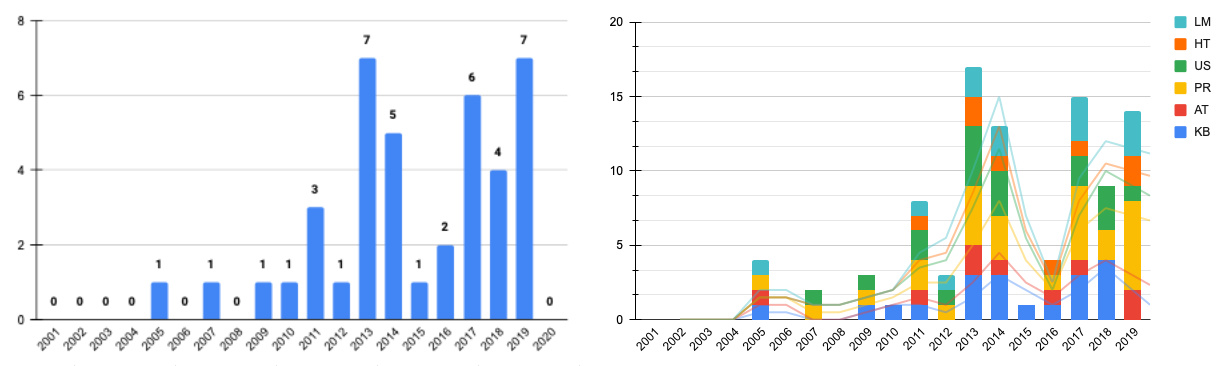
\includegraphics[width=16cm]{figures/doublechart.png}
    \caption{ \textbf{Left:} Number of articles published on AR piano within the last two decades. \textbf{Right:} Trend of contribution categories on the AR piano papers published within the last two decades. }
    \label{fig:doublechart}
\end{figure} 

The earliest prototype included in our systematic review was from the year 2005. However, while there have been patents and products filed on \textit{"augmented reality piano"} as early as the year 1998, which was before 2005, these were not included in the review because of the inclusion criteria described in subsection \ref{subsec: criteria}. Also, details that allow the author to review these patents systematically were not easily-accessible.

Between the years 2005 to 2010, along with the rise of mobile technologies and better phone cameras (especially the iPhone \cite{querashi2012apple}), a handful of studies have attempted to develop AR piano prototypes. These studies featured an virtual keyboard and piano roll notation that users can operate with. We can say that these contribution categories have been the earliest attempts to innovate piano learning with AR. We believe that the primary focus during these years, was to make piano learning exciting by introducing a \textit{"virtual"} keyboard that can be viewed anywhere. As the typical piano instrument is heavy and bulky, having augmented keyboards was the obvious and portable approach to begin with. As humans were slowly shifting from personal computing to mobile computing, the trend in piano learning was also headed towards the same direction.

Between the years 2011 to 2015, an obvious rise of AR piano prototypes published can be seen. The most common contributions during this period was the piano roll visualization. As mobile devices and their cameras were getting more powerful during this period, we believe that the focus may have shifted from bringing the classical piano into the mobile, to making the virtual keyboard more usable. Thus, user studies have to be utilized in order to assess this. Beyond usability, excitement and engagement were also key factors that need to be considered by these studies. Researchers had to innovate and introduce various learning modes to possibly make these user studies more realistic, and their results more accurate in relation to piano learning. Various use-cases and scenarios were introduced in user studies done by these papers. Practice modes, improving fingering accuracy, gamification and even supporting persons with disabilities (PWD's) were introduced. It was also in this period that the earliest known prototype to employ hand tracking \cite{huang2011piano} technology was also published. The work by \citet{weing2013piano} uses piano roll visualizations, employs hand tracking algorithms and introduces a gamified approach to learning modes for the users. Early use of agents and tutors as an addition to the augmented interfaces of the users were first introduced as well in these period. Similar to piano roll and learning modes, employing agents and tutors were embedded as part of interfaces that went beyond mobile. 3D technology was conceptualized were most utlized in the same period. The rise of the Kinect \cite{zhang2012microsoft} allowed human beings to interact beyond their mobile devices, moving towards surfaces and spaces. As such, hand and body tracking along with virtual tutors that \textit{"sit beside the learner"} were made possible with this technology. Some of these innovations pulled out the \textit{augmented} in mobile, and brought it to ubiquitous arena of ambient interfaces. With the use of Kinect and advanced 3D projectors \cite{yang2012augmented}, previously-solved problems on AR piano and spatial registration (in the mobile) have to be addressed when they were brought into  multidimensional spaces. 

\begin{figure}
    \centering
    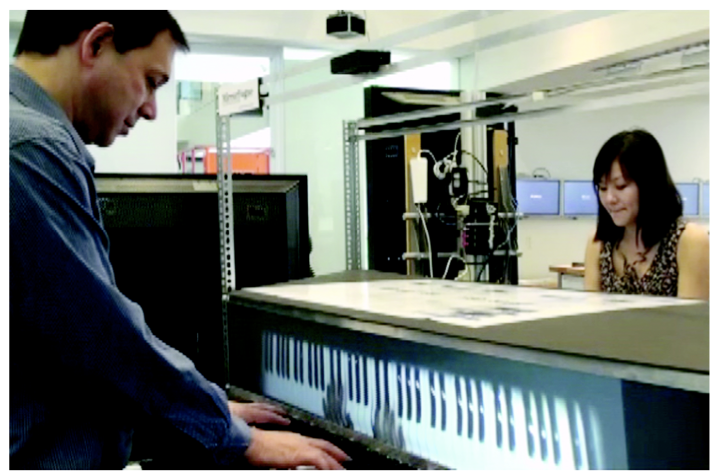
\includegraphics[width=7cm]{figures/xiaomrror2011.png}
    \caption{The work of \citet{xiao2011duet} introduced a virtual piano duet-partner that helped the piano learner in terms of pressing accuracy, posture, and sheet notation interpretation.}
    \label{fig:xiaomirror2011}
\end{figure}

Between the years 2016 to 2020, ubiquitous technologies (such us 3D, 360) have disrupted how contributions in AR. Piano roll visualizations, virtual keyboards and virtual agents have also been ported virtually-everywhere. As spatial registration in multidimensional space has been slowly addressed \cite{roberts2011spatial,novotny2013applications, billinghurst2008tangible} and applied in various environments, focus have shifted as well from mobile AR to tangible AR. Since keyboards, piano roll visualizations and agents can be displayed anywhere thanks to these innovations, humans still required tactile or haptic feedback when learning the piano. This was observed in the study of \citet{hamam2013effect} where he investigated on the kinesthetic and tactile feedback in relation to the quality of experience in using digital applications. Because AR piano technologies should not replace the classical piano, but rather augment the learning experience \cite{yang2020modern}, prototypes have to be developed in a way that makes the learning experience as similar as possible. This entails having or feeling the sensation as if the user is playing with the piano. The common trends have moved from having a virtual keyboard to having piano roll visualizations that guide the user on how to press realistic piano keys. Hand tracking technologies played a role in ensuring key-user press accuracy rather than matching virtual keys with user press. These piano prototypes have moved as well from individual learning experiences to considering remote, virtual or even multi-user collaborations. However, these prototypes did not have piano learning as a focus, instead they emphasized on piano performances. 



\section{Strategies in Designing AR Pianos}
\label{sec: strat}
\subsection{Hand Tracking}
something here 
\subsection{Visualisations}
Section discussing prototypes whose main contributions focused on visualizations, overlaying graphics, rendering and optimization etc
\subsection{Agents and Tutors}
Section discussing prototype whose main contributions focused on virtual agents/tutors 
\subsection{Learning Modes}
Section discussing prototype whose contributions focused on learning modes, emphasis on pedagogy and other learner-centric modes
\section{Evaluation Techniques}
done by studies on AR piano teaching systems (hypothesis based on cognition, realistic annotations etc)

% Please add the following required packages to your document preamble:
% \usepackage{graphicx}
\begin{table}[]
\caption{Table of Studies from \ref{tab:overview} with user studies. This table provides an overview of their techniques, treatments and tools used.}
\label{tab: us-all}
\resizebox{\textwidth}{!}{%
\begin{tabular}{lllllll} \hline \hline
\textbf{Ref.}                           & \textit{n}    & \textbf{treatment}    & \textbf{metrics constructs}    & \textbf{tools}\\ \hline
%P1 \cite{huang2011piano}              & 2011 &        & a                         & a                             & a                    \\
\cite{nugraha2014pemanfaatan}        & 8                & major and minor chords animated marker detection & usability, operation, attraction & self made questionnaire \\
\cite{chow2013music}                 & 7                & play a piece in the piano & usage, benefit, system rating & open ended questions \\
\cite{weing2013piano}                & 5                & practice and exploration modes & finger information, notation, satisfaction, cognitive load & self made questionnaire \\
\cite{kerdvibulvech2017innovative}  & 1                 & play a piece in the piano & scoring, time interval        & time tracking        \\
\cite{schmalstieg2007experiences}   & 0                 & a                         & a                             & a                    \\
\cite{correa2009computer}           & 0                 & a                         & a                             & a                    \\
\cite{takegawa2012piano}            & 0                 & a                         & a                             & a                    \\
\cite{xiao2010mirrorfugue}          & 0                 & a                         & a                             & a                    \\
\cite{xiao2013mirrorfugue}          & 0                 & a                         & a                             & a                    \\
\cite{li2018application}            & 0                 & a                         & a                             & a                    \\
\cite{leonard2013virtual}           & 0                 & a                         & a                             & a                    \\
\cite{raymaekers2014game}           & 0                 & a                         & a                             & a                    \\
\cite{rogers2014piano}              & 0                 & a                         & a                             & a                    \\
\cite{sun2018mr}                    & 0                 & a                         & a                             & a                    \\
\cite{molloy2019mixed}              & 0                 & a                         & a                             & a                    \\
\cite{pan2018pilot}                 & 0                 & a                         & a                             & a                    \\
\cite{kim2014ar}                    & 0                 & a                         & a                             & a                    \\
\cite{xiao2011duet}                 & 0                 & x                         & x                             & x                   \\ \hline 
                                    & \textit{\={x}}=6      &                      &                               &                   \\ \hline \hline 
\end{tabular}%
}
\end{table}




\section{Discussion and Future Directions}

gaps in modelling? position near your thesis

\section{Tables and Figures}
Figure of number of participants per study by years, size of each bubble is relative to sizes of other bubbles and based on number of participants in a study. Sort per category 

Table of AR piano teaching systems showing summary of survey
questionnaires

%\begin{figure}
%    \centering
%    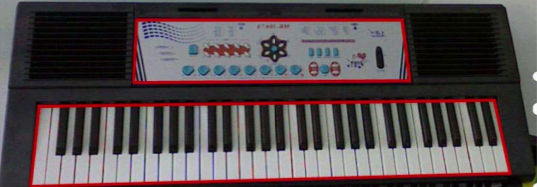
\includegraphics[width=7cm]{figures/pianomarker.png}
 %   \caption{Piano Augmented Reality marker}
 %   \label{fig:pianomarker}
%\end{figure}

%\begin{figure}
%    \centering
%    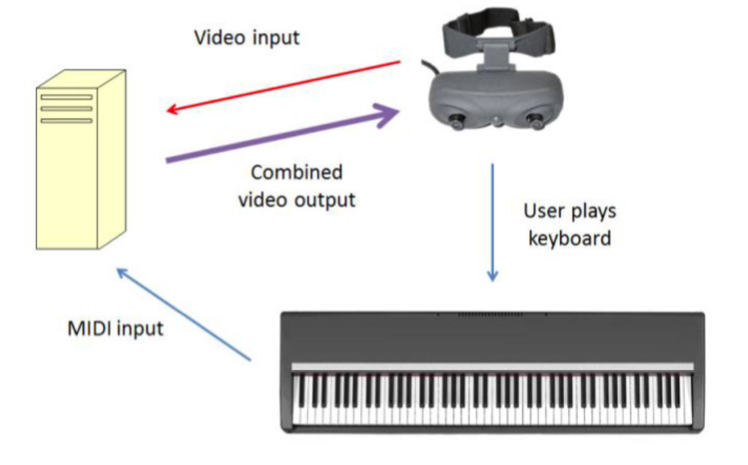
\includegraphics[width=7cm]{figures/headmountedpiano1.png}
 %   \caption{Architecture of the Head Mounted Piano by cite! }
%    \label{fig:pianoheadmountedarch}
%\end{figure}

%\begin{figure}
%    \centering
 %   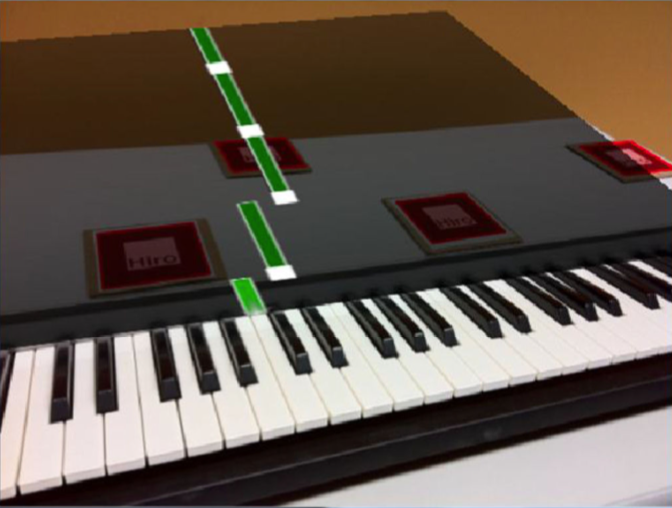
\includegraphics[width=7cm]{figures/headmountedview.png}
 %   \caption{View from the Head Mounted Piano AR  }
 %   \label{fig:View from the HeadMounted}
%\end{figure}

\begin{figure}
    \centering
    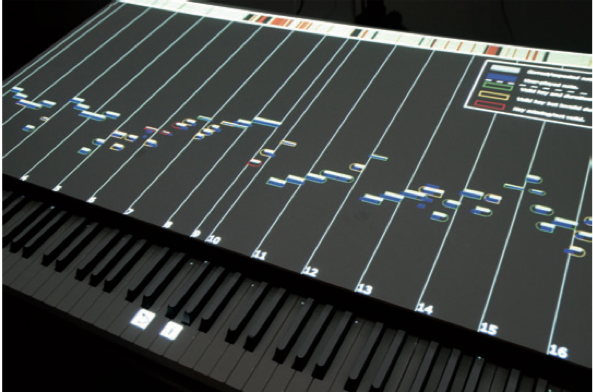
\includegraphics[width=7cm]{figures/piano}
    \caption{\cite{rogers2014piano}}
    \label{fig:rogers2014piano}
\end{figure}

\begin{figure}
    \centering
    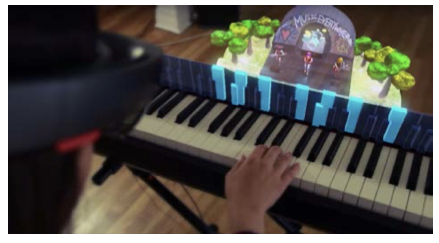
\includegraphics[width=7cm]{figures/daspiano.png}
    \caption{\cite{das2017music} }
    \label{fig:daspiano}
\end{figure}

\begin{figure}
    \centering
    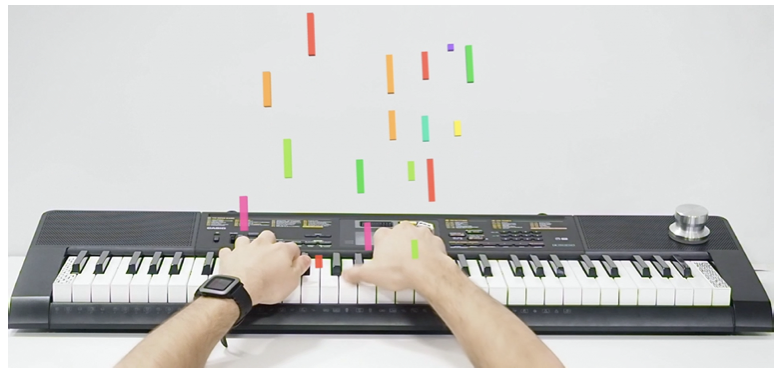
\includegraphics[width=15cm]{figures/arpianotrujano.png}
    \caption{\cite{trujano2018arpiano} }
    \label{fig:View from the HeadMounted}
\end{figure}

\begin{figure}
    \centering
    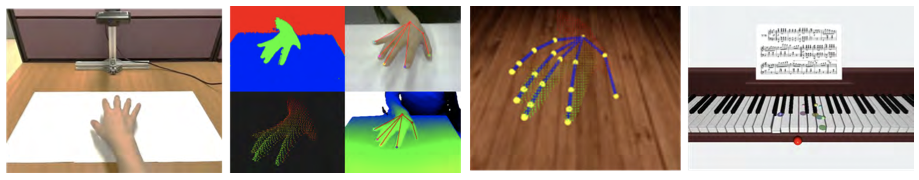
\includegraphics[width=15cm]{figures/lianghandtrack.png}
    \caption{\cite{liang2016barehanded} }
    \label{fig:View from the HeadMounted}
\end{figure}

\begin{figure}
    \centering
    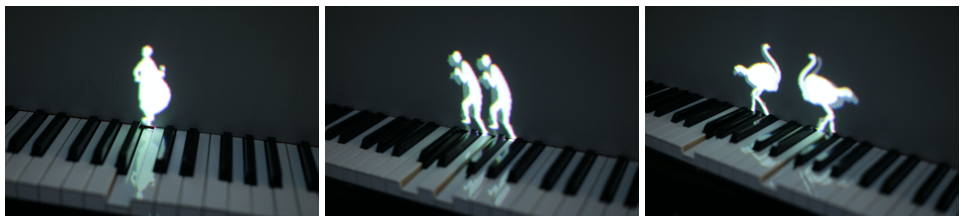
\includegraphics[width=15cm]{figures/xiaoandante.png}
    \caption{\cite{xiao2014andante} }
    \label{fig:View from the HeadMounted}
\end{figure}

\begin{figure}
    \centering
    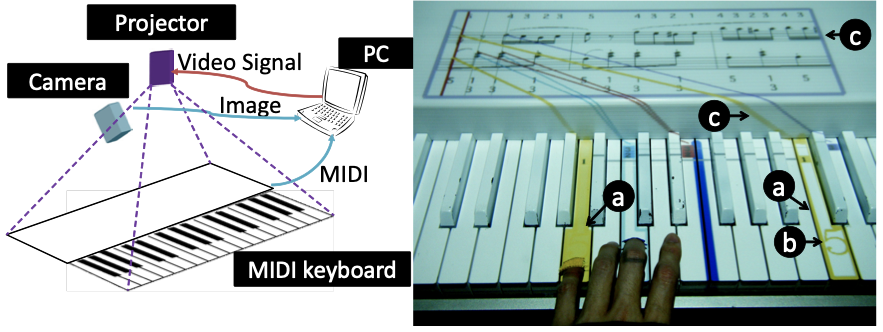
\includegraphics[width=15cm]{figures/takegawasetup.png}
    \caption{\cite{takegawa2012piano} }
    \label{fig:View from the HeadMounted}
\end{figure}

\begin{figure}
    \centering
    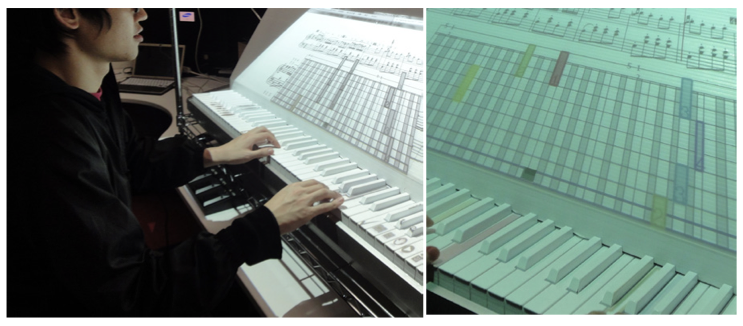
\includegraphics[width=15cm]{figures/takegawapianoroll.png}
    \caption{\cite{takegawa2012piano} }
    \label{fig:View from the HeadMounted}
\end{figure}

\begin{figure}
    \centering
    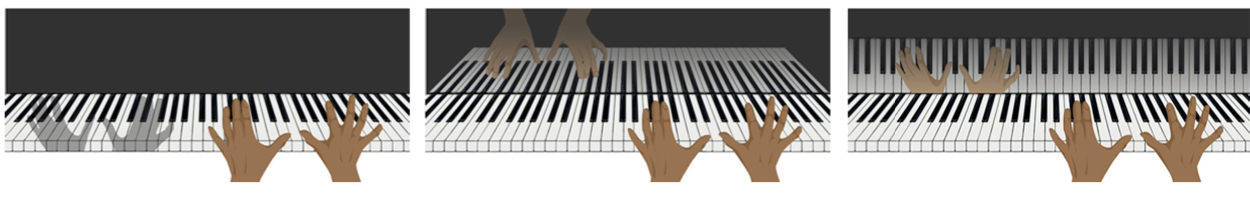
\includegraphics[width=15cm]{figures/xiaomirror3interfaces.png}
    \caption{\cite{xiao2010mirrorfugue} }
    \label{fig:View from the HeadMounted}
\end{figure}

\begin{figure}
    \centering
    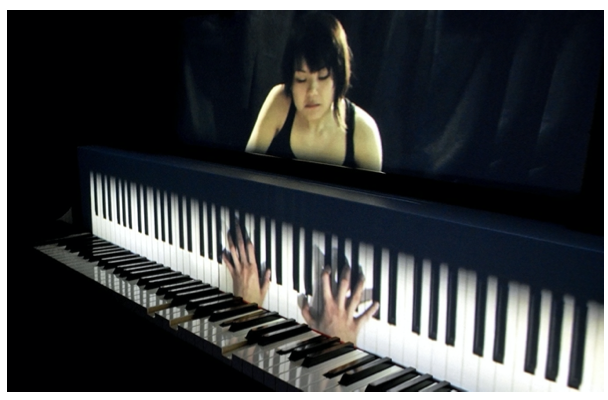
\includegraphics[width=7cm]{figures/xiaomirrorfugue3.png}
    \caption{\cite{xiao2013mirrorfugue} }
    \label{fig:xiao2013mirror}
\end{figure}

\begin{figure}
    \centering
    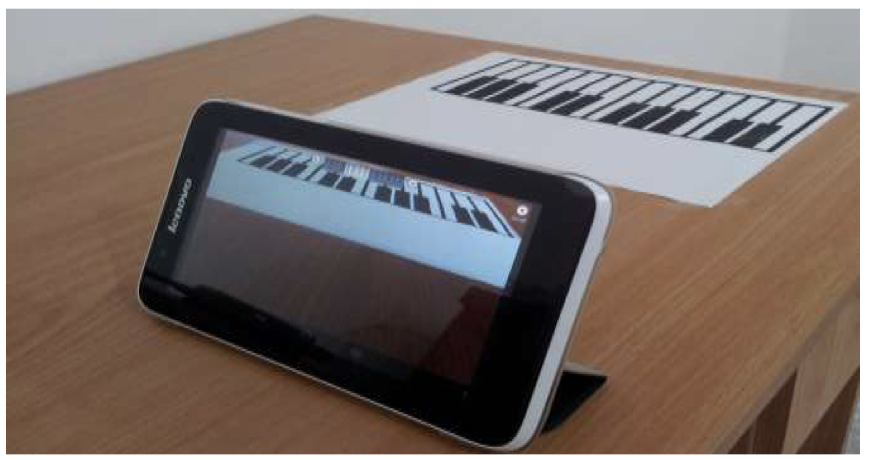
\includegraphics[width=7cm]{figures/zaqoutfingerpiano.png}
    \caption{\cite{zaqout2015augmented} }
    \label{fig:zaqoutfingerpiano}
\end{figure}

\begin{figure}
    \centering
    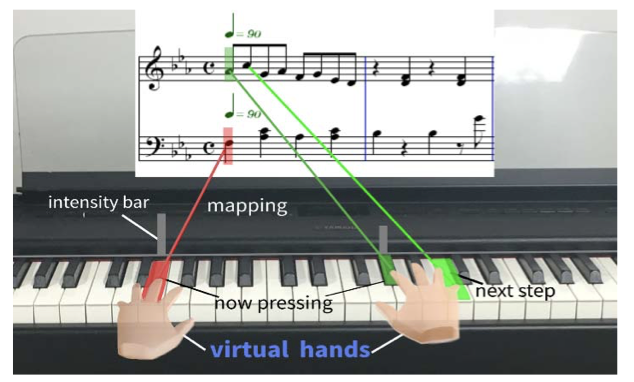
\includegraphics[width=7cm]{figures/caipiano.png}
    \caption{\cite{cai2019designa} }
    \label{fig:caipiano}
\end{figure}


\begin{figure}
    \centering
    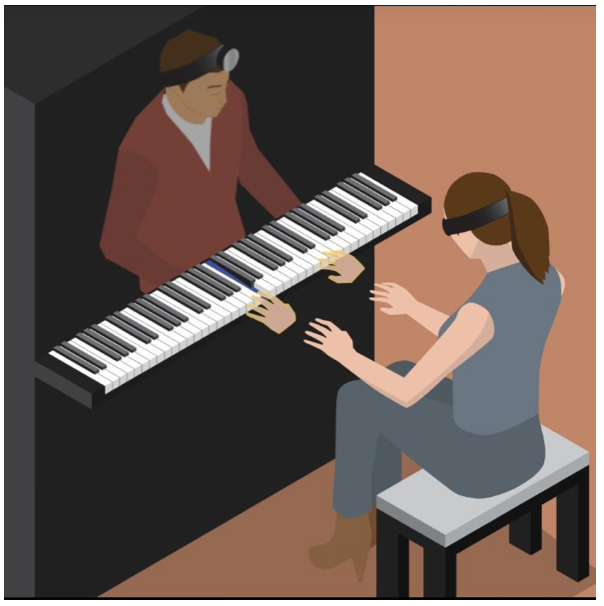
\includegraphics[width=7cm]{figures/gerryadept.png}
    \caption{\cite{gerry2019adept} }
    \label{fig:gerryadept}
\end{figure}

\begin{figure}
    \centering
    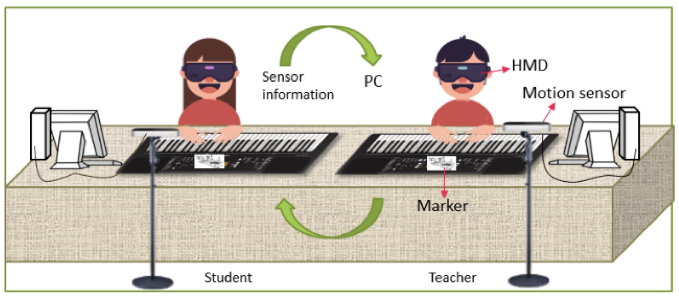
\includegraphics[width=7cm]{figures/caigroup.png}
    \caption{\cite{cai2019designb} }
    \label{fig:caigroup}
\end{figure}


%%
%% The next two lines define the bibliography style to be used, and
%% the bibliography file.
\bibliographystyle{ACM-Reference-Format}
\bibliography{sample-base}
%%
%\nocite{*}
%% If your work has an appendix, this is the place to put it.
%\appendix
\end{document}
\endinput
%%
%% End of file `sample-manuscript.tex'.
